\chapter{Counting number of partitions into independent sets}
\label{chap:num-partitions-into-indep-sets}

Recall that in table \ref{tab:platonic-exactly-n-clrs} we count two colorings $c_1$ and $c_2$ as different also in the case, when $c_1$ can be obtained as a permutation of colors of $c_2$. This is something we would like to avoid if we are interested in the structure of the coloring only, and the values of the colors have no special meaning.

\begin{defn}[relabeling relation]\label{dfn:relabeling-relation}
    Given a graph $G=(V,E)$ and a set of colorings $C$, we define a relation $\leftrightarrow \; \subseteq C \times C$ as follows: For any two colorings $c_1,c_2 \in C$ we have $c_1 \leftrightarrow c_2$ iff exists a permutation of colors $\pi$ s.t. $\forall v \in V : c_1(v) = \pi(c_2(v))$. We call this relation the \emph{relabeling relation}.
\end{defn}

The relabeling relation is in fact an equivalence relation, as it is reflexive, symmetric and transitive.

\begin{defn}[number of exact n-partitions]
    Let us for a given $n \in \mathbb{N}$ denote by $P^*_{\leftrightarrow}(G,n)$ the number of equivalence classes of $\leftrightarrow$ on the set of all proper vertex colorings using exactly $n$ colors. 
\end{defn}

The equivalence classes in definition above correspond to different partitions of the set $V(G)$ into independent sets irrespectively of the particular colors that we assign the vertices. Note that now, we might still consider two partitions as different even though they can be made equal by applying some automorphism. 

In order to calculate $P^*_{\leftrightarrow}(G,n)$, consider any partition $W$ of $V(G)$ into independent sets and count how many different colorings correspond to $W$. Because $W$ consists of exactly $n$ independent sets, we have $n!$ possible ways of assigning colors to the independent sets of $W$. As this holds for any arbitrary partition of size $n$, it follows that:
\begin{equation}\label{eqn:count-relabel-orbits}
    P^*_{\leftrightarrow}(G,n) \cdot n! = P^*(G,n)
\end{equation}

Using this formula, we can compute yet another table shown below:

\begin{table}[H]
\centering
\begin{tabular}{l@{\hspace{0.5cm}}ccccccc}
\toprule
\textbf{Platonic solid} & \textbf{2} & \textbf{3} & \textbf{4} & \textbf{5} & \textbf{6} & \textbf{7} & \textbf{8} \\
\midrule
tetrahedron & $0$ & $0$ & $1$ & $0$ & $0$ & $0$ & $0$ \\
octahedron & $0$ & $1$ & $3$ & $3$ & $1$ & $0$ & $0$ \\
cube & $1$ & $18$ & $92$ & $146$ & $80$ & $16$ & $1$ \\
icosahedron & $0$ & $0$ & $10$ & $660$ & $4908$ & $10008$ & $7900$ \\
dodecahedron & $0$ & $1200$ & $7019920$ & $\approx 10^{8}$ & $\approx 10^{10}$ & $\approx 10^{11}$ & $\approx 10^{11}$ \\
\bottomrule
\end{tabular}
\caption{Numbers of of possible partitions of vertices of the graphs into $n$ independent sets.}
\label{tab:platonic-exact-n-partitions}
\end{table}

Notice, that even though we managed to overcome the problem of counting a single partition $W$ of $G$ into independent sets multiple times, because of the ways we can relabel the colorings, the method still suffers from the following: Rotated or reflected independent sets might be counted as different objects. This happens exactly in cases, when by rotating some partition $W_1$, we arrive at a partition $W_2$ s.t. for any coloring $c_1$ obtained by labeling the sets of $W_1$ and for any coloring $c_2$ obtained by labeling sets of $W_2$ we have $c_1 \not\leftrightarrow c_2$. In other words, we cannot construct coloring $c_2$ just by renaming the colors of coloring $c_1$ or vice versa.

This problem is illustrated on figure \ref{fig:example-octahedron-4-partitions} below. We can see that all three partitions are same when we allow rotating the solid. But it is impossible to obtain one coloring from another by simply relabeling the colors. 

\begin{figure}[H]
    \centering
    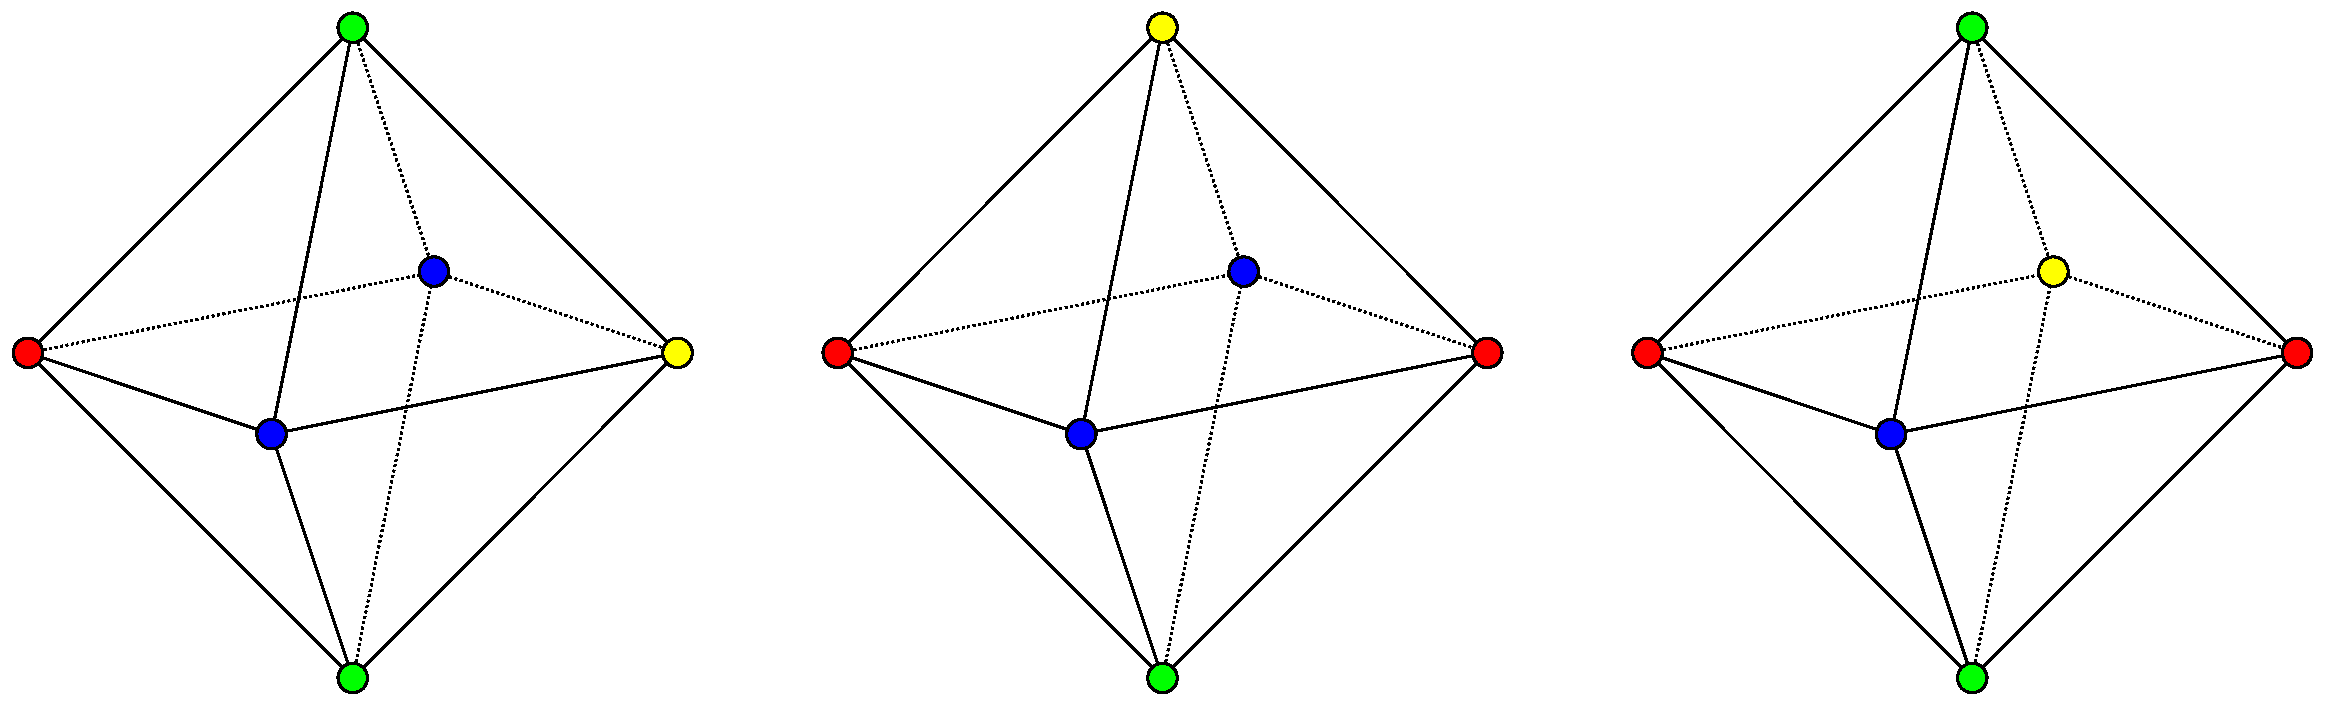
\includegraphics[width=1\textwidth]{Resources/Figs/example-octahedron-4-partitions.pdf}
    \caption{All partitions of octahedron to 4 independent sets. Notice that they are structurally equivalent when we allow us to rotate the solid.}
    \label{fig:example-octahedron-4-partitions}
\end{figure}

Note that in some cases of symmetric colorings, this problem is avoided. For example, any rotation or reflection of a 4-coloring of tetrahedron can be obtained by simply relabeling the colors as well. See this on the figure below:

\begin{figure}[H]
    \centering
    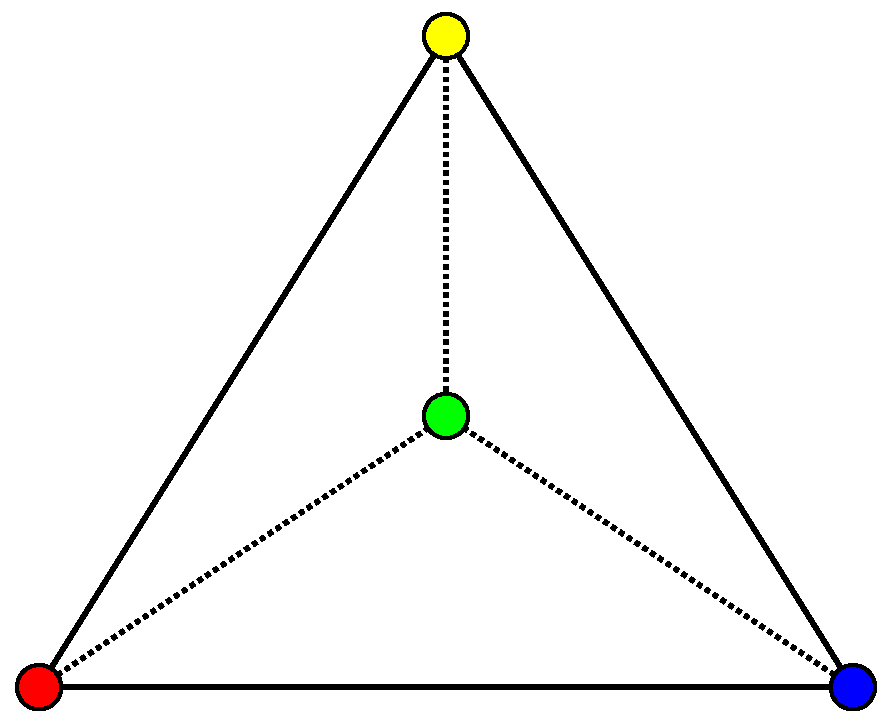
\includegraphics[width=0.3\textwidth]{Resources/Figs/example-tetrahedron-4-clring.pdf}
    \caption{A coloring of tetrahedron using 4 colors. Notice that any rotation of this coloring can be obtained by simply relabeling the colors.}
    \label{fig:example-tetrahedron-4-coloring}
\end{figure}

Overcoming the problem, of counting rotations or reflection of the same partition multiple times, motivates the following definition:

\begin{defn}[relabeling-automorphism relation]\label{dfn:relabeling-automorphism-relation}
    Let $G=(V,E)$ be a graph and $C$ a set of its vertex colorings. We define a relation $\rightleftharpoons \; \subseteq C \times C$ as follows: Given two colorings $c_1,c_2 \in C$ we have $c_1 \rightleftharpoons c_2$ iff there exists a permutation of colors $\pi$ and an automorphism $\alpha \in \Aut(G)$ s.t. $\forall v \in V : c_1(v) = \pi(c_2(\alpha(v)))$. We call this relation the \emph{relabeling-automorphism relation}.
\end{defn}

The relabeling-automorphism relation is again an equivalence relation. 

For reflexivity, we can simply take $\pi = id$ and $\alpha = id$. For symmetry, suppose we have $\pi$ and $\alpha$ s.t. $\forall v \in V : c_1(v) = \pi(c_2(\alpha(v)))$. Suppose we have a $w \in V$, then there exists $v \in V$ s.t. $w = \alpha(v)$. We will show that $c_2(w) = \pi^{-1}(c_1(\alpha^{-1}(w)))$. We can substitute for $w$ to get $c_2(\alpha(v)) = \pi^{-1}(c_1(\alpha^{-1}(\alpha(v))))$ which is equivalent to $c_2(\alpha(v)) = \pi^{-1}(c_1(v)) \iff c_1(v) = \pi(c_2(\alpha(v)))$ which holds by the assumption. For transitivity, we have that $\exists \pi, \pi', \alpha ,\alpha'$ s.t. $\forall v \in V : c_1(v) = \pi(c_2(\alpha(v))) \wedge c_2(v) = \pi'(c_3(\alpha'(v)))$. By substituting for $c_2(\alpha(v))$ into the left operand of the previous conjunction we get $c_1(v)=\pi(\pi'(c_3(\alpha'(\alpha(v)))))$. This means that $\pi \circ \pi'$ and $\alpha' \circ \alpha$ are the permutation of colors and automorphism respectively, by which $c_1 \rightleftharpoons c_3$.

Thus, since $\rightleftharpoons$ is an equivalence relation, we can again consider its partition into equivalence classes, $C/_\rightleftharpoons$ and count the number of these classes, $\abs{C/_\rightleftharpoons}$. This is an interesting number to calculate, since if $C$ is the set of n-colorings of graph $G$, then each equivalence class corresponds to a structurally different partition of $V(G)$ into $n$ non-empty independent sets.

\begin{defn}[orbital number of exact n-partitions]
    Let us for a given $n \in \mathbb{N}$ denote by $P^*_{\rightleftharpoons}(G,n)$ the number of equivalence classes of $\rightleftharpoons$ on the set of all proper vertex colorings using exactly $n$ colors. 
\end{defn}

It is tempting to suppose, that $P^*_{\rightleftharpoons}(G,n)$ can be calculated from $OP^*(G,n)$ in a similar fashion as can $P^*_{\leftrightarrow}(G,n)$ be calculated using $P^*(G,n)$ by formula \ref{eqn:count-relabel-orbits}. In order to prove that formula, we showed, that for each equivalence class of $C/_\leftrightarrow$, we count exactly $n!$ colorings in $C$ when we use $P^*(G,n)$. If something similar is to hold for $\rightleftharpoons$, we would have to show, that for each equivalence class of $C/_\rightleftharpoons$, we count exactly $k$ equivalence classes of $C/_\sim$ when using $OP^*(G,n)$, for some fixed number $k$. Unfortunately, this is not the case since there exists graph $G$ and a set of its n-colorings $C$ s.t. there are equivalence classes of $C/_\rightleftharpoons$ that are counted exactly once by $OP^*(G,n)$, but also classes that are counted multiple times.

For example, consider the graph of cube and its following two 4-colorings:

\begin{figure}[H]
    \centering
    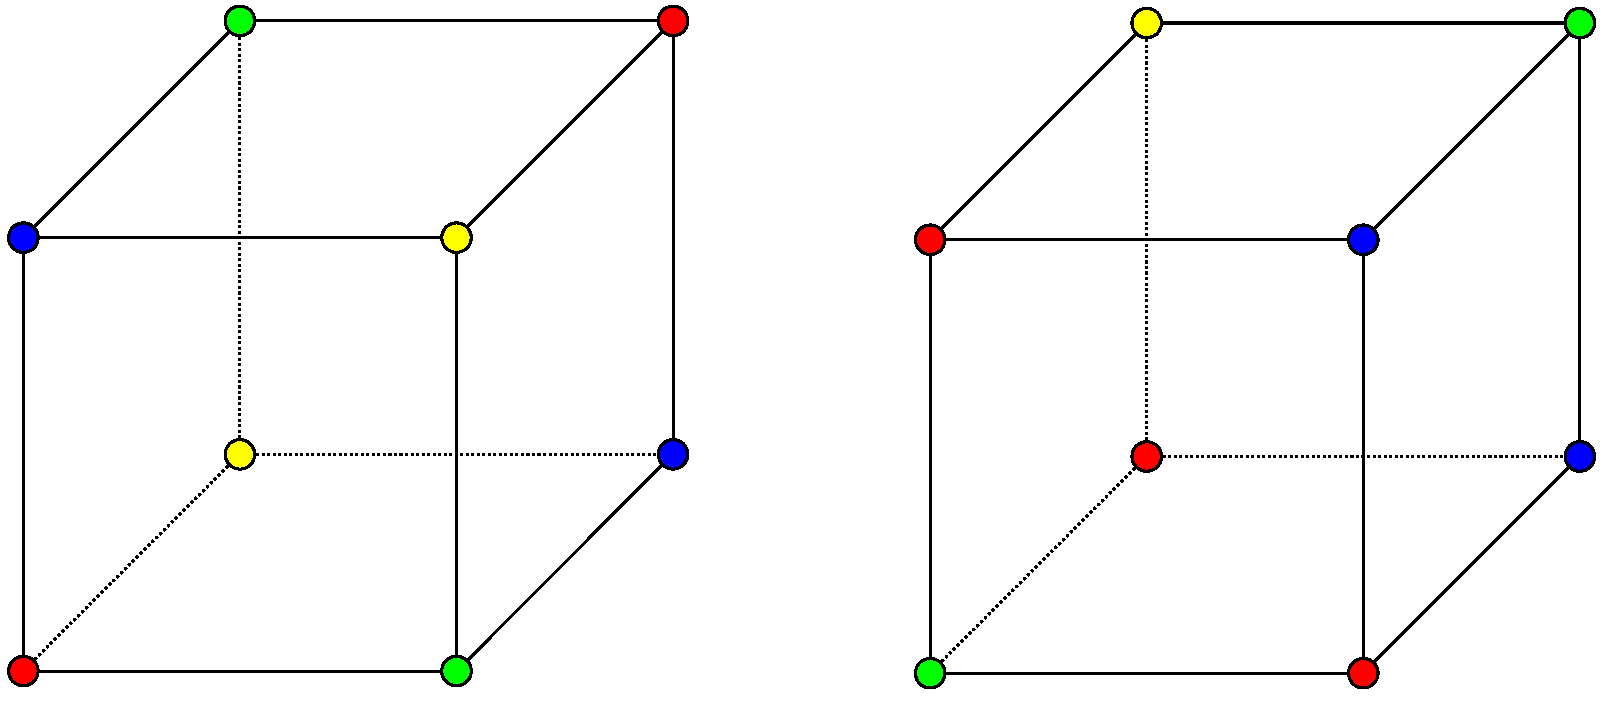
\includegraphics[width=0.75\textwidth]{Resources/Figs/example_diff_rel-aut_class_sizes.pdf}
    \caption{Two colorings s.t. each represents a single class of $\rightleftharpoons$ relation. Any possible relabeling of colors of the left coloring corresponds to a single class of $\sim$ relation. On the other hand any relabeling of colors of the right coloring belongs to a different equivalence class of $\sim$.}
    \label{fig:example-cube-4-clrings-diff-classes}
\end{figure}

When the colorings in figure \ref{fig:example-cube-4-clrings-diff-classes} are viewed as a partition, then the left partition represents a single equivalence class of both $\sim$ and $\rightleftharpoons$. This follows from the fact, that permuting the colors of the independent set leads to a coloring, that can be obtained from the original coloring by simply rotating the solid as well.

On the other hand, the partition on the right represents $4!$ equivalence classes of $\sim$, since any permutation of colors yields a different equivalence class of $\sim$.

\section{Simple bounds on number of equivalence classes of the relabeling-automorphism relation}

Before we show, how the number of equivalence classes of $\rightleftharpoons$ can be computed using an enumerative algorithm, we provide bounds on the this number, $P^*_\rightleftharpoons(G,n)$, using numbers $P^*_\leftrightarrow(G,n)$ or $OP^*(G,n)$.

\begin{claim}\label{clm:relabeling-bound}
    For any graph $G=(V,E)$ and a natural number $n$, we have: $$\frac{1}{\abs{\Aut(G)}} \cdot P^*_\leftrightarrow(G,n) \leq P^*_\rightleftharpoons(G,n) \leq P^*_\leftrightarrow(G,n)$$ 
\end{claim}

\begin{proof}

The inequality $P^*_\rightleftharpoons(G,n) \leq P^*_\leftrightarrow(G,n)$ is simple. It follows from the fact, that for any two colorings $c_1$,$c_2$ of graph $G$, if we have $c_1 \not\rightleftharpoons c_2$, then also $c_1 \not\leftrightarrow c_2$. So there must be at least as many equivalence classes of $\leftrightarrow$ as they are of $\rightleftharpoons$.

For inequality $\frac{1}{\abs{\Aut(G)}} \cdot P^*_\leftrightarrow(G,n) \leq P^*_\rightleftharpoons(G,n)$ we show, that for each equivalence class of $\rightleftharpoons$ there are at most $n!$ equivalence classes of $\leftrightarrow$. Remember, that $n$ is the number of colors, i.e. independent sets, that the considered colorings use. Let $c_1$ be some coloring, that belongs to some equivalence class $E_\rightleftharpoons$ of $\rightleftharpoons$ and equivalence class $E_\leftrightarrow$ of $\leftrightarrow$. All possible relabelings of colors of $c_1$ will be contained in both classes $E_\rightleftharpoons$ and $E_\leftrightarrow$. On the other hand, there exist at most $\abs{\Aut(G)}$ ways to rotate the coloring $c_1$, all of which will be contained in $E_\rightleftharpoons$, but may result in at most $\abs{\Aut(G)}$ different equivalence classes of $\leftrightarrow$.

\end{proof}

Notice, that the result of claim $\ref{clm:relabeling-bound}$ gives us equality for any graph $G$ s.t. $\Aut(G) = \{id\}$ i.e. a graph, whose only symmetry is the identity function. In general, the lower bound is higher for graphs that are not very symmetric. Unfortunately, this is not the case for our graphs, so the lower bounds will not give us as much information as they could, for different classes of graphs.

See below examples of bounds calculated using formulas from claim \ref{clm:relabeling-bound}:

\begin{table}[H]
\centering
\begin{tabular}{l@{\hspace{0.5cm}}ccccccc}
\toprule
\textbf{Platonic solid} & \textbf{2} & \textbf{3} & \textbf{4} & \textbf{5} & \textbf{6} & \textbf{7} & \textbf{8} \\
\midrule
tetrahedron & $0$ & $0$ & $1$ & $0$ & $0$ & $0$ & $0$ \\
 & $0$ & $0$ & $1$ & $0$ & $0$ & $0$ & $0$ \\
\specialrule{0.2pt}{0.65ex}{0.65ex}
octahedron & $0$ & $1$ & $3$ & $3$ & $1$ & $0$ & $0$ \\
 & $0$ & $1$ & $1$ & $1$ & $1$ & $0$ & $0$ \\
\specialrule{0.2pt}{0.65ex}{0.65ex}
cube & $1$ & $18$ & $92$ & $146$ & $80$ & $16$ & $1$ \\
 & $1$ & $1$ & $2$ & $4$ & $2$ & $1$ & $1$ \\
\specialrule{0.2pt}{0.65ex}{0.65ex}
icosahedron & $0$ & $0$ & $10$ & $660$ & $4908$ & $10008$ & $7900$ \\
 & $0$ & $0$ & $1$ & $6$ & $41$ & $84$ & $66$ \\
\specialrule{0.2pt}{0.65ex}{0.65ex}
dodecahedron & $0$ & $1200$ & $7019920$ & $\approx 10^{8}$ & $\approx 10^{10}$ & $\approx 10^{11}$ & $\approx 10^{11}$ \\
 & $0$ & $10$ & $58500$ & $7761169$ & $\approx 10^{8}$ & $\approx 10^{9}$ & $\approx 10^{9}$ \\
\bottomrule
\end{tabular}
\caption{Upper and lower bounds for the number of equivalence classes of the relabeling-automorphism relation based on the number of equivalence classes of the relabeling relation. For each solid, top row contains the upper bounds while bottom row contains the lower bounds.}
\label{tab:bounds-exactn-n-partitions}
\end{table}

\begin{claim}\label{clm:automorphism-bound}
    For any graph $G=(V,E)$ and a natural number $n$, we have: $$\frac{1}{n!} \cdot OP^*(G,n) \leq P^*_\rightleftharpoons(G,n) \leq OP^*(G,n)$$
\end{claim}

\begin{proof}

Argument for inequality $P^*_\rightleftharpoons(G,n) \leq OP^*(G,n)$ is again simple and analogous to the one in clam \ref{clm:relabeling-bound}. We notice, that if for any two colorings $c_1,c_2$ we have $c_1 \not\rightleftharpoons c_2$ then also $c_1 \not\sim c_2$.

For inequality $\frac{1}{n!} \cdot OP^*(G,n) \leq P^*_\rightleftharpoons(G,n)$ we proceed again analogously as in claim \ref{clm:relabeling-bound}. We show that for each equivalence class of $\rightleftharpoons$, we have at most $n!$ equivalence classes of $\sim$ corresponding to that class. We imagine a coloring $c_1$ that belongs to some equivalence class $E_\rightleftharpoons$ of $\rightleftharpoons$ and $E_\sim$ of $\sim$. Applying any automorphism $\alpha \in \Aut(G)$ results in a coloring, that will be contained in both $E_\rightleftharpoons$ and $E_\sim$. On the other hand, by relabeling the colors of $c_1$, we may obtain $n!$ colorings s.t. each belongs to a different equivalence class of $\sim$ even though they all belong to $E_\rightleftharpoons$.

\end{proof}

Note, that the lower bound resulting from claim $\ref{clm:automorphism-bound}$ is useful for cases where $n$, the number of colors, is small. In such cases, it can give us a better bound than what the bound from claim $\ref{clm:relabeling-bound}$ gives.

See upper and lower bounds resulting from claim \ref{clm:automorphism-bound} in table \ref{tab:bounds-orbital} below.

\begin{table}[H]
\centering
\begin{tabular}{l@{\hspace{0.5cm}}ccccccc}
\toprule
\textbf{Platonic solid} & \textbf{2} & \textbf{3} & \textbf{4} & \textbf{5} & \textbf{6} & \textbf{7} & \textbf{8} \\
\midrule
tetrahedron & $0$ & $0$ & $1$ & $0$ & $0$ & $0$ & $0$ \\
 & $0$ & $0$ & $1$ & $0$ & $0$ & $0$ & $0$ \\
\specialrule{0.2pt}{0.65ex}{0.65ex}
octahedron & $0$ & $1$ & $6$ & $15$ & $15$ & $0$ & $0$ \\
 & $0$ & $1$ & $1$ & $1$ & $1$ & $0$ & $0$ \\
\specialrule{0.2pt}{0.65ex}{0.65ex}
cube & $1$ & $12$ & $100$ & $485$ & $1290$ & $1680$ & $840$ \\
 & $1$ & $2$ & $5$ & $5$ & $2$ & $1$ & $1$ \\
\specialrule{0.2pt}{0.65ex}{0.65ex}
icosahedron & $0$ & $0$ & $2$ & $660$ & $29454$ & $420336$ & $2654400$ \\
 & $0$ & $0$ & $1$ & $6$ & $41$ & $84$ & $66$ \\
\specialrule{0.2pt}{0.65ex}{0.65ex}
dodecahedron & $0$ & $75$ & $1404548$ & $\approx 10^{8}$ & $\approx 10^{11}$ & $\approx 10^{12}$ & $\approx 10^{14}$ \\
 & $0$ & $13$ & $58523$ & $7761220$ & $\approx 10^{8}$ & $\approx 10^{9}$ & $\approx 10^{9}$ \\
\bottomrule
\end{tabular}
\caption{Upper and lower bounds for the number of equivalence classes of the relabeling-automorphism relation based on the number of equivalence classes of the $\sim$ relation. For each solid, top row contains the upper bounds while bottom row contains the lower bounds.}
\label{tab:bounds-orbital}
\end{table}

\section{Algorithm for computing number of equivalence classes of the relabeling-automorphism relation}\label{sec:equiv-classes-of-relaut}

For all the algorithms below, let $n$ be the number of colors of colorings we consider. The colorings are represented as lists of integers ranging from $1$ to $n$, where $n$ is the number of colors. The lists are indexed by vertices, which are numbers $1, \ldots,|V|$.

Since we are dealing with graphs that have relatively small amount of edges and vertices, we can compute some of the numbers using a simple algorithm that works by first enumerating all coloring and then filtering the ones that are equivalent. The algorithm can be split into the following two parts:

\subsection{Finding representatives of the relabeling relation}

First, we want to exclude colorings, that correspond to the same partitions into independent sets, but just have different labels for the colors. This corresponds to finding colorings that represent different classes of the relabeling relation from definition \ref{dfn:relabeling-relation}. To do so, we use the fact, that the colorings are represented as lists together with the following observation: Given a partition into $n$ independent sets, there are $n!$ ways to assign labels to the colorings. Out of these $n!$ colorings, there is always exactly one coloring s.t. it is in a so called \textit{canonic form}.  

\begin{defn}[canonic form]\label{dfn:canonic-form}
    Let $B=\{1,\ldots,n\}$ be a set of colors and $c$ be a coloring using colors $B$ s.t. $c$ is represented as sequence $(b_1, \ldots,b_{\abs{V}})$ s.t. $\forall i: b_i \in B$. For each $i \in B$, denote $k_i$ the lowest index at which color $i$ appears. We say that $c$ is in \emph{canonic form} if $\forall i < j \in B: k_i < k_j$.
\end{defn}

In other words, a coloring is in canonic form, if when we go through the coloring from lowest index to highest index, we encounter the colors for the first time in the same order as what their values are. Now the observation is as follows: For all $n!$ ways to assign colors to the independent sets, there is exactly one coloring s.t. it is in canonic form. This means, that by keeping only the colorings in canonic form, we get exactly colorings representing the equivalence classes of the relabeling relation.

\begin{algorithm}[H]
    \caption{Algorithm for testing whether a given coloring is in canonic form by definition \ref{dfn:canonic-form}.} 
    \begin{algorithmic}[1]
        \Function{IsInCanonicForm}{$c$}
            \State $k \gets 1$      
            \For{color $b_i$ in coloring $c$}
                \If{$b_i > k$}
                    \State \Return False
                \EndIf
                 \If{$b_i = k$}
                    \State $k \gets k + 1$
                \EndIf
            \EndFor   
            \State \Return True
        \EndFunction
    \end{algorithmic}
    \label{alg:is-in-canonic-form}
\end{algorithm}

\subsection{Finding representatives of relabeling-automorphism relation}

By filtering the colorings that are not in canonic form, we have reduced the number of colorings we need to deal with by a factor of $n!$. After performing that step, we can proceed with a more computationally heavy \todo[JF, noinline]{? "demanding"} part of the algorithm. In this part of the algorithm, we go through the colorings we were left with, and build a set $R$ of representatives of the relabeling-automorphism class. In each step, when we consider some next coloring $c_i$, we compare $c_i$ with all representatives in $R$, that we have found so far. If $c_i$ can be unified by an automorphism with some representative $r_j \in R$, then we continue to the next coloring. Otherwise, we add $c_i$ to $R$ i.e. we declare $c_i$ as a representative of its $\rightleftharpoons$ class. See the detailed description of the algorithm below:

\begin{algorithm}[H]
    \caption{Algorithm for finding representatives of equivalence classes of the relabeling-automorphism relation as defined in \ref{dfn:relabeling-automorphism-relation}. $G$ is a graph and $C$ is the set of colorings in canonic form.} 
    \begin{algorithmic}[1]
        \Function{FindRelabelingAutomorphismRepresentatives}{$G,C$}
            \State $R \gets \emptyset$
            \For{coloring $c_i \in C$}
                \For{coloring $r_j \in R$}
                    \If{$c_i$ and $r_j$ can be unified by some $\alpha \in \Aut(G)$ and relabeling}
                        \State Continue with next coloring at step 3
                    \EndIf
                \EndFor
                \State $R \gets R \cup \{c_i\}$
            \EndFor
            \State \Return $R$
        \EndFunction
    \end{algorithmic}
    \label{alg:representatives-of-relabeling-automorphism-relation}
\end{algorithm}

Using this algorithm, we can ask for size of set $R$, to get the number of equivalence classes of the $\rightleftharpoons$ relation. Since step $5$ of the algorithm above is a bit more involved, we describe it in more detail below. We use notation $\Dom(\pi)$ and $\Rng(\pi)$ to describe the domain and range of function $\pi$ respectively. Also, we treat each cycle $O$ of an automorphism $\alpha$ as a sequence of vertices $(v_1,\ldots,v_k)$, where $k := \abs{O}$. See description of the algorithm below:

\begin{algorithm}[H]
    \caption{Algorithm testing if two colorings $c_1, c_2$ can be unified by given automorphism $\alpha$ by some relabeling \pi.} 
    \begin{algorithmic}[1]
        \Function{TestRelabelingAutomorphismRelated}{$c_1,c_2,\alpha$}
            \State $\pi \gets \emptyset$
            \For{cycle $O \in \alpha$}
                \State $k \gets \abs{O}$
                \For{$v_i \in O$}
                    \If{$c_1(v_i ) \notin \Dom(\pi)$}
                        \If{$c_2(v_{i + 1 \bmod k}) \notin \Rng(\pi)$}
                            \State $\pi(c_1(v_i)) \gets c_2(v_{i + 1 \bmod k})$
                        \Else
                            \State \Return False
                        \EndIf
                    \Else
                        \If{$\pi(c_1(v_i )) \neq c_2(v_{i + 1 \bmod k})$}
                            \State \Return False
                        \EndIf
                    \EndIf
                \EndFor
            \EndFor
            \State \Return True
        \EndFunction
    \end{algorithmic}
    \label{alg:test-two-colorings-relabel-automorph-related}
\end{algorithm}

In natural language, the algorithm above tries to construct a mapping $\pi$ from colors of coloring $c_1$ to colors of coloring $c_2$. This mapping must be a valid permutation of colors, so we require that no two colors from $c_1$ map to a single color in $c_2$.

Step $5$ of algorithm \ref{alg:representatives-of-relabeling-automorphism-relation} consists of testing, whether for some $\alpha \in \Aut(G)$, the algorithm \ref{alg:test-two-colorings-relabel-automorph-related} above returns True.

See next section for results we computed using the algorithm above.

\section{Numbers of equivalence classes of relabeling-automorphism relation}\label{sec:nums-equiv-classes-relaut}

In this section, we provide tables with values of $P^*_\rightleftharpoons(G,n)$, which we managed to compute. It is especially interesting, to compare results in tables below with the results we got in tables \ref{tab:platonic-chrompolys-exacts} and \ref{tab:archimedean-chrompolys-exacts}. We can see, that the numbers reduced significantly.

Unfortunately, we can also see, that there are some entries in the tables left out, for which the algorithm took too long to get the resulting number.\todo[JF, noinline]{dám Vám komentář osobně, jak to napsat; v mezidobí, zkuste třeba sage na HPC a více času} Note, that we did not have this issue when computing tables \ref{tab:platonic-chrompolys-exacts} and \ref{tab:archimedean-chrompolys-exacts}, since we were already provided with the chromatic polynomial, which we could simply evaluate at certain points. By doing that, we avoided having to enumerate all colorings, which is the most computationally heavy part of the algorithm from section \ref{sec:equiv-classes-of-relaut}.

\begin{table}[H]
\centering
\begin{tabular}{l@{\hspace{0.5cm}}ccccccc}
\toprule
\textbf{Platonic solid} & \textbf{2} & \textbf{3} & \textbf{4} & \textbf{5} & \textbf{6} & \textbf{7} & \textbf{8} \\
\midrule
tetrahedron & $0$ & $0$ & $1$ & $0$ & $0$ & $0$ & $0$ \\
octahedron & $0$ & $1$ & $1$ & $1$ & $1$ & $0$ & $0$ \\
cube & $1$ & $3$ & $9$ & $10$ & $7$ & $2$ & $1$ \\
icosahedron & $0$ & $0$ & $1$ & $12$ & $\cdot$ & $\cdot$ & $\cdot$ \\
dodecahedron & $0$ & $17$ & $\cdot$ & $\cdot$ & $\cdot$ & $\cdot$ & $\cdot$ \\
\bottomrule
\end{tabular}
\caption{Calculated numbers of equivalence classes of the $\rightleftharpoons$ relation of Platonic solids using the algorithm above. The symbol $\cdot$ means that the computation took longer than 60 seconds and hence was terminated.}
\label{tab:plat-nums-relabeling-automorphism-classes}
\end{table}

\begin{table}[H]
\centering
\begin{tabular}{l@{\hspace{0.5cm}}ccccccc}
\toprule
\textbf{Archimedean solid} & \textbf{2} & \textbf{3} & \textbf{4} & \textbf{5} & \textbf{6} & \textbf{7} & \textbf{8} \\
\midrule
truncated tetrahedron & $0$ & $2$ & $119$ & $\cdot$ & $\cdot$ & $\cdot$ & $\cdot$ \\
cuboctahedron & $0$ & $2$ & $24$ & $\cdot$ & $\cdot$ & $\cdot$ & $\cdot$ \\
truncated cube & $0$ & $65$ & $\cdot$ & $\cdot$ & $\cdot$ & $\cdot$ & $\cdot$ \\
truncated octahedron & $1$ & $\cdot$ & $\cdot$ & $\cdot$ & $\cdot$ & $\cdot$ & $\cdot$ \\
\bottomrule
\end{tabular}
\caption{Calculated numbers of equivalence classes of the $\rightleftharpoons$ relation of selected Archimedean solids using the algorithm above. The symbol $\cdot$ means that the computation took longer than 60 seconds and hence was terminated.}
\label{tab:arch-nums-relabeling-automorphism-classes}
\end{table}

\section{Visualizing relabeling-automorphism classes of selected solids}

In this section, we would like to interpret the results from section \ref{sec:nums-equiv-classes-relaut}, by showing the colorings, that represent the equivalence classes we counted.

\todo[JF]{zmiňte, že je budete ilustrovat jen na několika jednoduchých podle tabulky 6.4 a přitom netriviálních (tedy ne na všech), třeba je v té tabulce barevně vyznačte a v caption zmiňte, to to vyznačení znamená}

For many cases, we have multiple equivalence classes for particular values of $n$, where $n$ is the number of independent sets in the partition. In such cases, we will organize the respective partitions in following figures by a so called \textit{size sequence}.

\begin{defn}[size sequence]
    Let $G=(V,E)$ be a graph and let $W$ be a partition of $V$ into $n$ independent sets, where $n$ is some natural number. Let $s=(\abs{I_1}, \ldots, \abs{I_n})$ be a vector s.t. $\forall i: I_i \in W$, $\forall i \neq j: I_i \neq I_j$ and $\forall i \leq j : \abs{I_i} \leq \abs{I_j}$. We call this the \emph{size sequence} of partition $W$.
\end{defn}

In other words, the size sequence is an ordered sequence of sizes of the independent sets in $W$.

\subsection{Octahedron relabeling-automorphism classes}

For octahedron, we can observe, that for any number of colors ranging from $3$ to $6$, its graph has only a single partition into independent sets, up to symmetries. See the four corresponding figures below:

\begin{figure}[H]
    \centering
    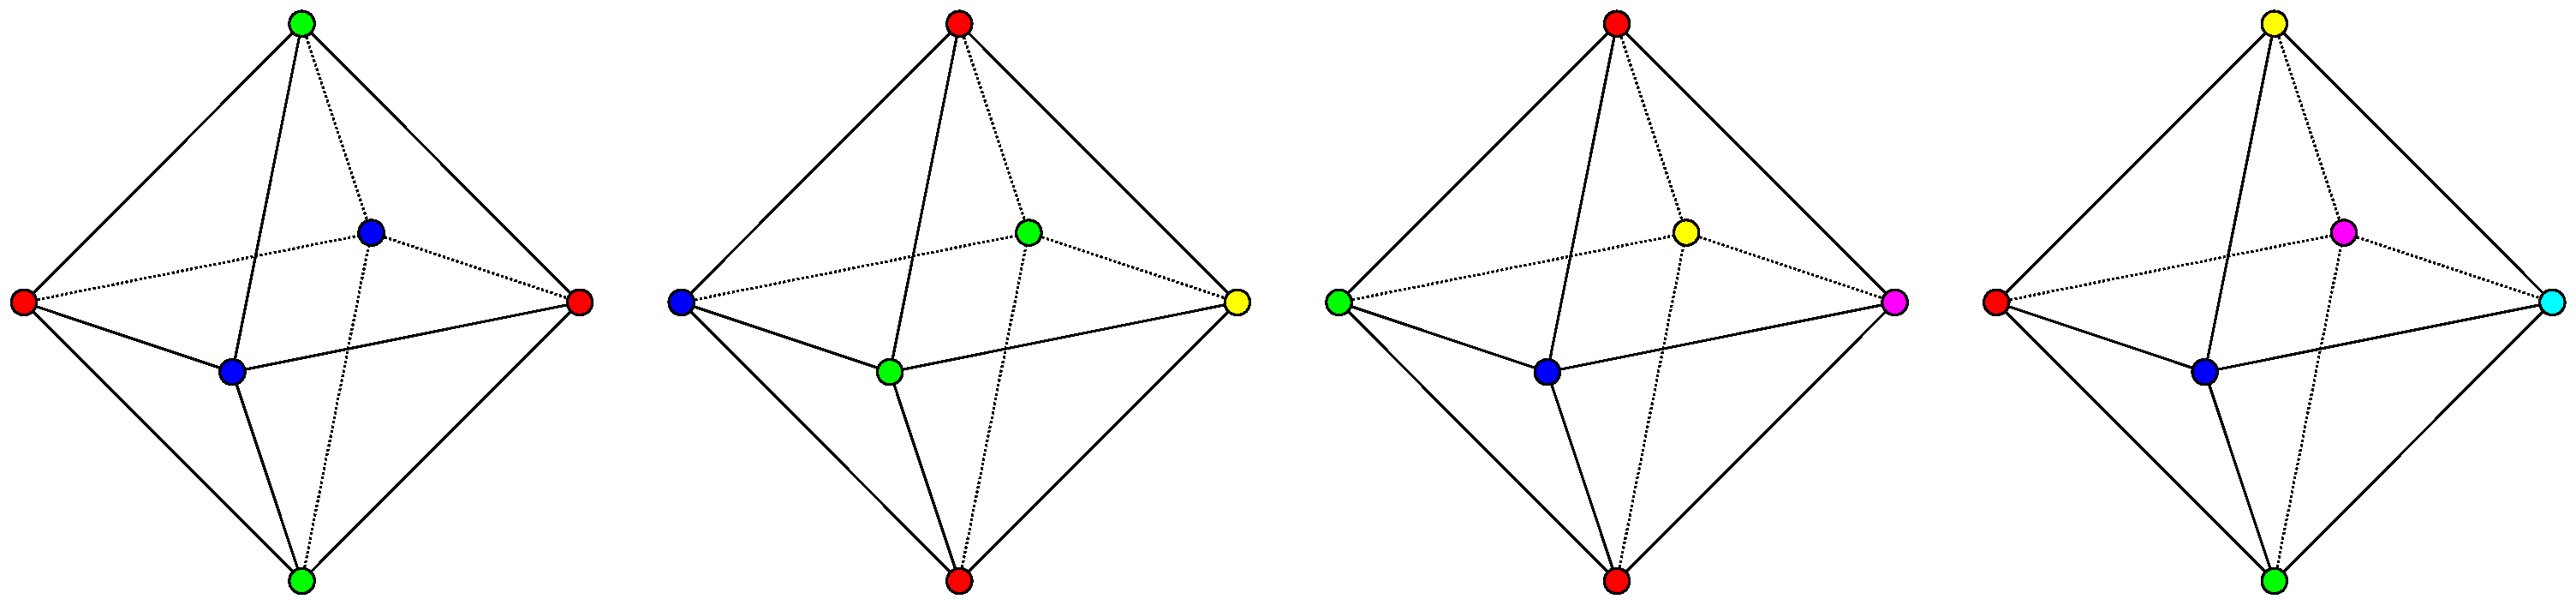
\includegraphics[width=1\textwidth]{Resources/Figs/octahedron-relaut-classes.pdf}
    \caption{Equivalence classes of relabeling-automorphism of octahedron for $n$ from $3$ up to $6$.}
    \label{fig:octahedron-relaut-classes}
\end{figure}

\todo[JF]{Možná by už tu bylo dobré zrovna ilustrovat size sequence, přímo pod obrázky.}

\subsection{Cube relabeling-automorphism classes}

In the case of cube and $n=3$, we have three non-equivalent partitions s.t. their size sequences are pairwise different. See the following figure: 

\begin{figure}[H]
    \centering
    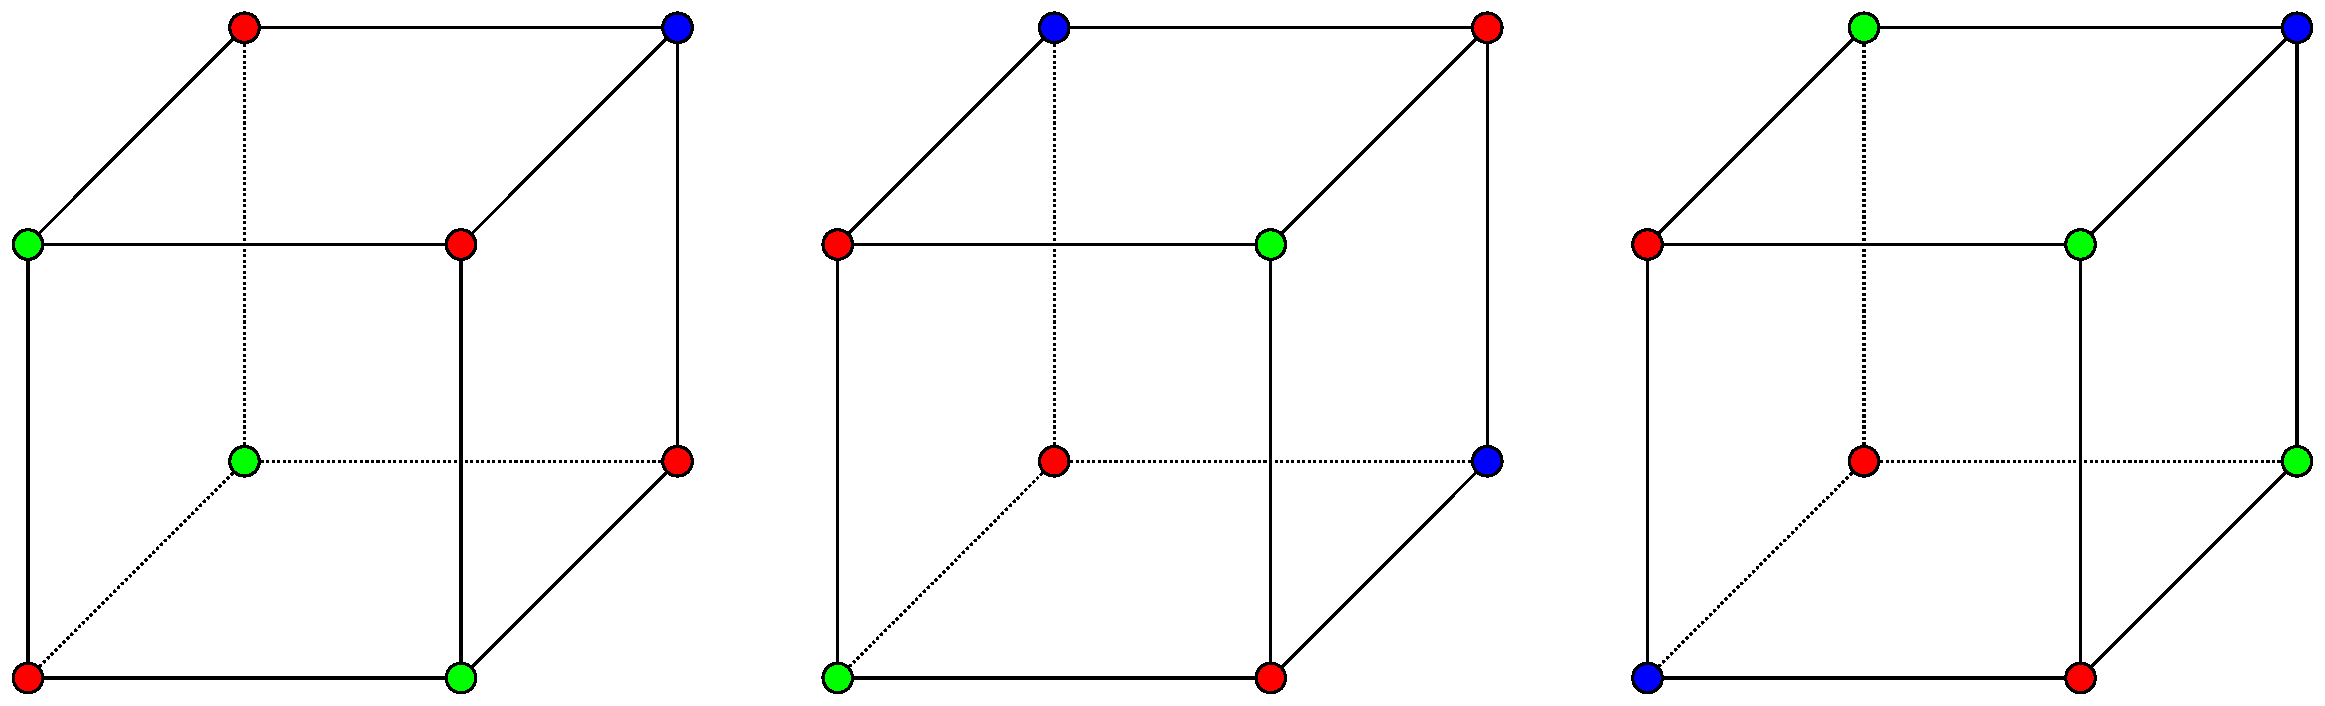
\includegraphics[width=1\textwidth]{Resources/Figs/cube_non_relaut-3-clrings.pdf}
    \caption{Equivalence classes of relabeling-automorphism relation of cube for $n=3$. The size sequences are $(1,3,4), (2,2,4)$ and $(2,3,3)$ respectively.}
    \label{fig:cube-3clring-relaut-classes}
\end{figure}

For $n=4$, the situation is a bit more interesting. This comes from the fact, that now we have size sequences, to which correspond multiple non-equivalent partitions into independent sets. In total, we have $9$ partitions. See figure below:

\begin{figure}[H]
    \centering
    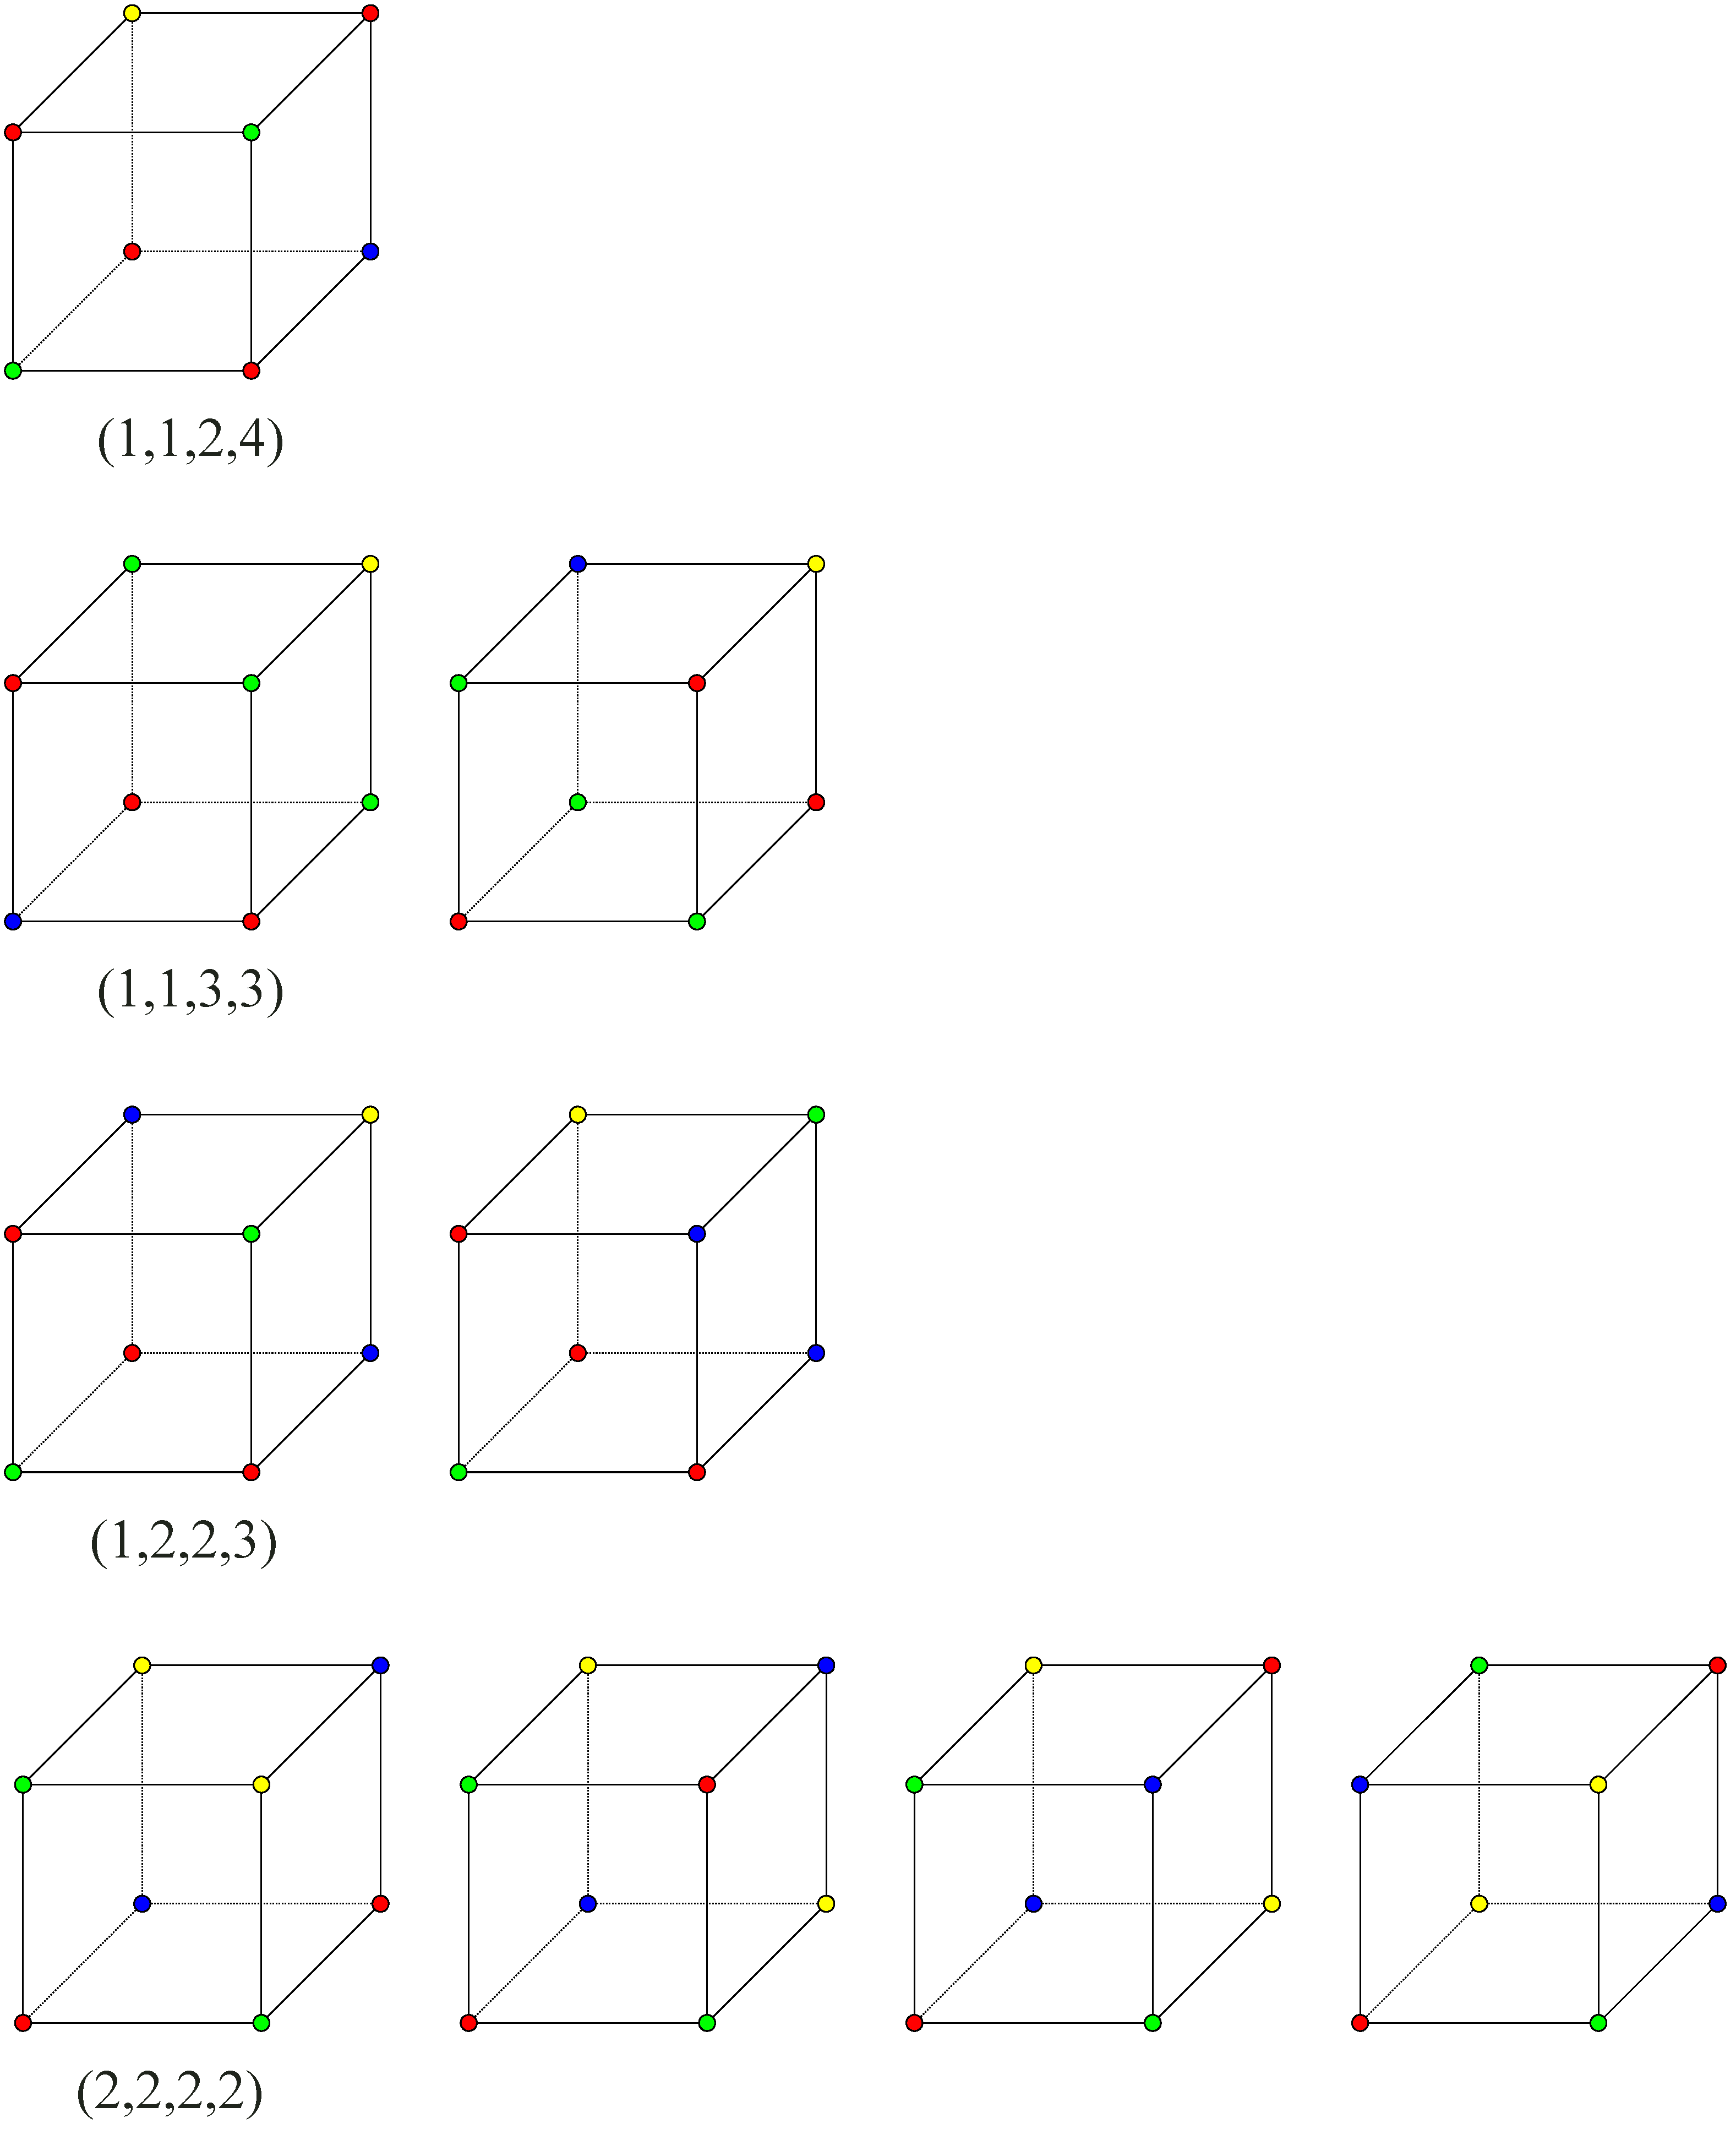
\includegraphics[width=1\textwidth]{Resources/Figs/cube_non_relaut-4-clrings.pdf}
    \caption{Equivalence classes of relabeling-automorphism relation of cube for $n=4$. The size sequences of the rows are $(1,1,2,4)$, $(1,1,3,3)$, $(1,2,2,3)$ and $(2,2,2,2)$ going from top to bottom.}
    \label{fig:cube-4clring-relaut-classes}
\end{figure}

Last specific example, we would like to show on cube, is for $n=7$. In that case, we are allowed to have only a single independent set of size $2$, which we will call $T$, and all other sets must be singletons. From this observation follows, that the number of orbits is equal to all non-equivalent ways, in which we can arrange the vertices in $T$. Since vertices in $T$ must be non-adjacent, they can either be across the face diagonal or the space diagonal. Thus, we have two possible non-equivalent arrangements, which are shown below:

\begin{figure}[H]
    \centering
    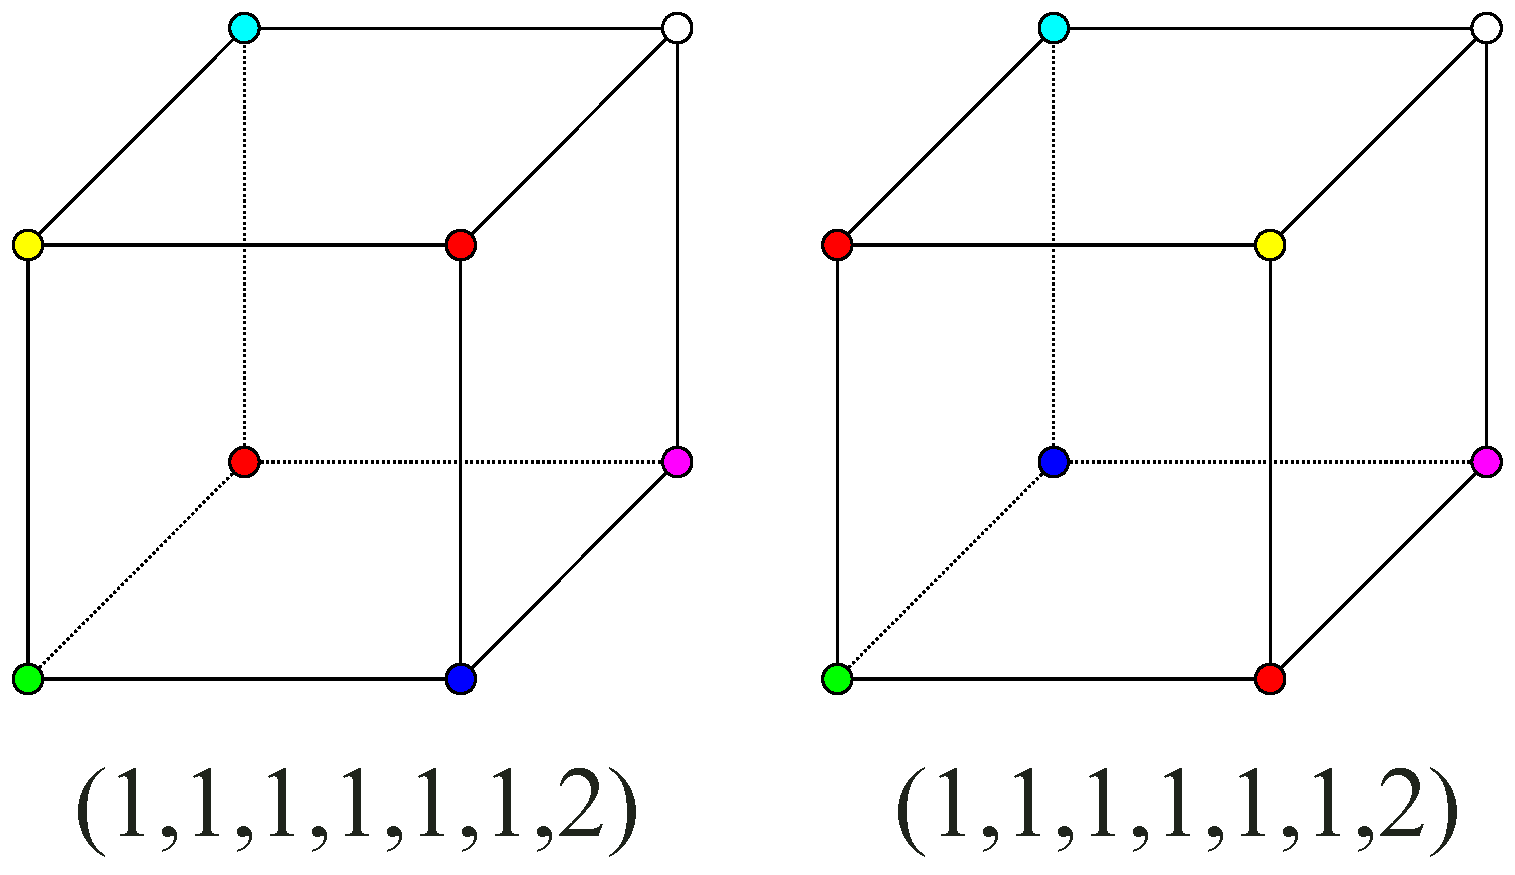
\includegraphics[width=0.75\textwidth]{Resources/Figs/cube_non_relaut-7-clrings.pdf}
    \caption{The only two equivalence classes of relabeling-automorphism relation of cube for $n=7$ that exist. They correspond exactly to the different ways, in which we can position the two red vertices s.t. they are non-adjacent.}
    \label{fig:cube-7clring-relaut-classes}
\end{figure}

\subsection{Icosahedron relabeling-automorphism classes}

For icosahedron and $n=4$, it turns out that there is only the following equivalence class:

\begin{figure}[H]
    \centering
    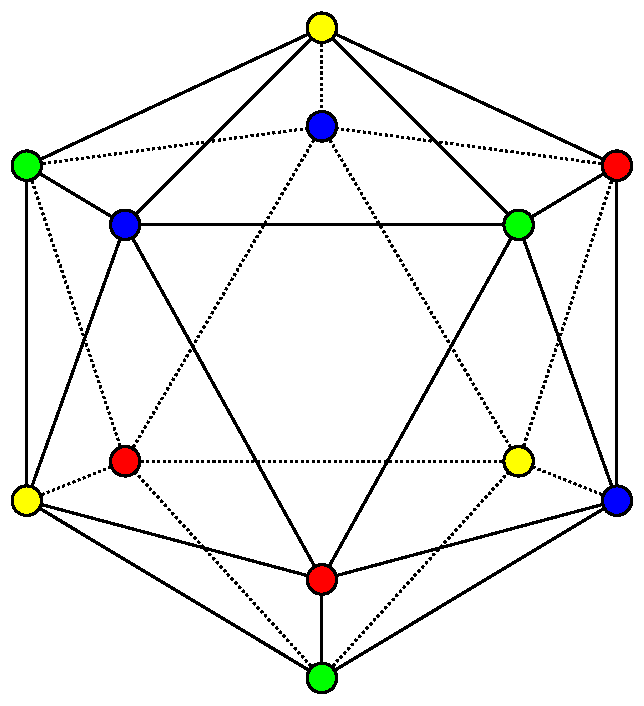
\includegraphics[width=0.4\textwidth]{Resources/Figs/icosahedron_non_relaut-4-clrings.pdf}
    \caption{The only equivalence class of the relabeling-automorphism relation of icosahedron for $n=4$.}
    \label{fig:icosahedron-4clring-relaut-classes}
\end{figure}

